\section{Reconstruction de l'image}

Une fois le masque appliqué à l'image, nous sommes ramené à un problème dit d'\emph{inpainting}. Il s'agit alors de trouver une méthode permettant de combler les trous formés par le masquage en respectant la structure de l'image. Il existe de nombreuses méthodes pour cela, après quelques expérimentations nous avons sélectionné une méthode d'\emph{inpainting} par régularisation parcimonieuse - avec un seuillage de type \emph{soft} et des ondelettes orthogonales. 




%\subsection{Inpainting par régularisation variationnelle}
%
%\subsubsection{Inpainting avec norme Sobolev}
%
%La résolution du problème d'inpainting repose sur un problème de minimisation d'énergie - ici norme de Sobolev - sous des contraintes de correspondance. Ainsi si on note $Phi$ l'opérateur de masquage de l'image - avec le masque extrait - et $y$ l'image masquée, l'\emph{inpainting} par Sobolev se récrit :
%\begin{equation}
%f^* = \arg \min E(f) = \|\nabla f \|^2 \text{ sous contraintes } \Phi(f) = y
%\end{equation}
%Cette fonction à minimiser est régulière et l'on peut utiliser un algorithme de descente de gradient projeté. Si l'on note - $\Omega$ est le masque :
%\begin{equation}
%(\Pi f)_i = 
%\left\{
%\begin{array}{lll}
%y_i & \text{si} & i\in\Omega \\
%f_i & \text{si} & i\notin\Omega
%\end{array}
%\right.
%\end{equation}
%l'opérateur de projection orthogonal sur la contrainte $Phi f = y$, alors l'algorithme de descente de gradient projeté consiste à itérer : 
%\begin{equation}
%f^{(n+1)} = \Pi \left( f^{(n)} + \tau \Delta(f^{(n)})\right)
%\end{equation}
%où $\Delta = - \nabla^* \circ \nabla$ (l'adjoint du gradient étant -div. Le terme de mise à jour est donc bien le terme classique de gradient dans la descente de gradient - ici c'est le gradient de l'énergie de Sobolev $E(f)$. La condition de convergence de la méthode de descente de gradient projetée est que le pas de mise à jour vérifie : 
%\begin{equation}
%\tau < \frac{2}{\|\Delta \|}
%\end{equation}
%
%Les résultats de l'\emph{inpainting} avec norme de Sobolev sont présenté en figure (A METTRE). INTERPRETATION.
%
% 
%\subsubsection{Inpainting avec norme TV}
%
%On peut aussi remplacer dans le problème d'optimisation précédent la norme de Sobolev par la norme de variation totale (TV). Nous verrons qu'elle a tendance à mieux reconstruire les contours que la norme Sobolev qui floute les images. Pour autant elle n'est pas différentiable en 0, on lui préfère donc sa version régularisée :
%\begin{equation}
%J_{\epsilon}(f) = \sum_x \sqrt{\|\nabla f(x) \|^2 + \epsilon^2}
%\end{equation}
%De nouveau on peut réutiliser l'algorithme de descente de gradient projeté, il suffit donc de calculer le gradient de cette nouvelle énergie. Il vaut : 
%\begin{equation}
%G_{\epsilon} = - \text{div} \left( \frac{(\nabla f)_i}{\sqrt{\| (\nabla f)_i \|^2 + \epsilon^2}}\right)_i
%\end{equation}
%La contrainte à respecter sur le pas est cette fois-ci :
%\begin{equation}
%\tau < \frac{\epsilon}{4}
%\end{equation}
%(RESULTATS + INTERPRETATION).
%
%
%\subsection{Inpainting par régularisation parcimonieuse}

La méthode d'\emph{inpainting} par régularisation parcimonieuse diffère des méthodes classique de régularisation variationnelle - qui minimisent une énergie, soit Sobolev soit TV en pratique - en ce sens qu'elle passe par une représentation parcimonieuse de l'image avant d'essayer de combler les trous. La représentation considérée est engendrée par une base de vecteurs $\Psi = (\psi_m)_m$, usuellement une base d'ondelette. Les coefficients dans cette base sont noté $a =(a_m)_m$, on par du principe que la représentation est parcimonieuse - \emph{i.e.} les $(a_m)_m$ le sont. On cherche un ensemble de coefficients $a^*$ qui résout :
\begin{equation}
a^* \in \arg \min_a \frac{1}{2} \| y - \Phi \Psi a \|^2 + \lambda J(a)
\end{equation}
Le paramètre $\lambda$ correspond à de la régularisation pour le bruit, comme nos images ne sont pas bruitée, nous prenons un $\lambda$ très faible. La notation $\Psi a = \sum_m a_m \psi_m$ indique uniquement l'opération de reconstruction du signal. Souvent on prend $J(a)$ comme la norme $L^1$ : $J(a) = \sum_m \|a_m \|$.

On note $S^{\Psi}(a)$ la fonction de seuillage - \emph{soft} ou \emph{hard} - dans la base $\Psi$. On peut prendre plusieurs bases d'ondelettes, nous présenterons des résultats pour une base orthogonale et une autre invariante par translation. L'algorithme utilisé pour résoudre le problème de minimisation précédent est le \emph{forward-backward splitting} - aussi connu comme \emph{iterative thresholding}. Il s'agit d'itérer : 
\begin{equation}
f^{(n+1)} = S^{\Psi}_{\tau,\lambda}(f^{(n)} - \tau \Phi^*(\Phi f^{(n)} - y) )
\end{equation}
L'avantage de prendre des ondelettes orthogonales est que $\Phi^* = \Phi$. Dans ce cas, pour qu'il y ait convergence le pas doit vérifier :
\begin{equation}
\tau < \frac{2}{\| \Phi^* \Phi \|} = 2
\end{equation}
Avec $\tau = 1$, et des ondelettes orthogonales toujours, l'étape de descente de gradient revient à projeter sur la contrainte $\mathcal{C} = \{f | \forall \Omega(x) = 1, f(x) = y(x) \}$. Ainsi dans le cas d'ondelettes orthogonales, l'algorithme revient à :
\begin{equation}
f^{(n+1)} = S_{\lambda}^{\Psi} (\text{Proj}_{\mathcal{C}} (f^{(n)}))
\end{equation}
Cet algorithme s'adapte dans le cas d'ondelette non orthogonales mais les dernières simplifications ne sont plus licites. 

Dans notre cas, bien que le SNR soit plus élevé avec des méthodes type variationnelles (en particulier avec la norme TV), nous avons préféré ce type d'\emph{inpainting} avec un seuillage doux et des ondelettes orthogonales car le rendu visuel est le cohérent. Nous en montrons quelques résultats en Fig.(\ref{ee}).

\begin{figure}
\centering
\begin{tabular}{cc}
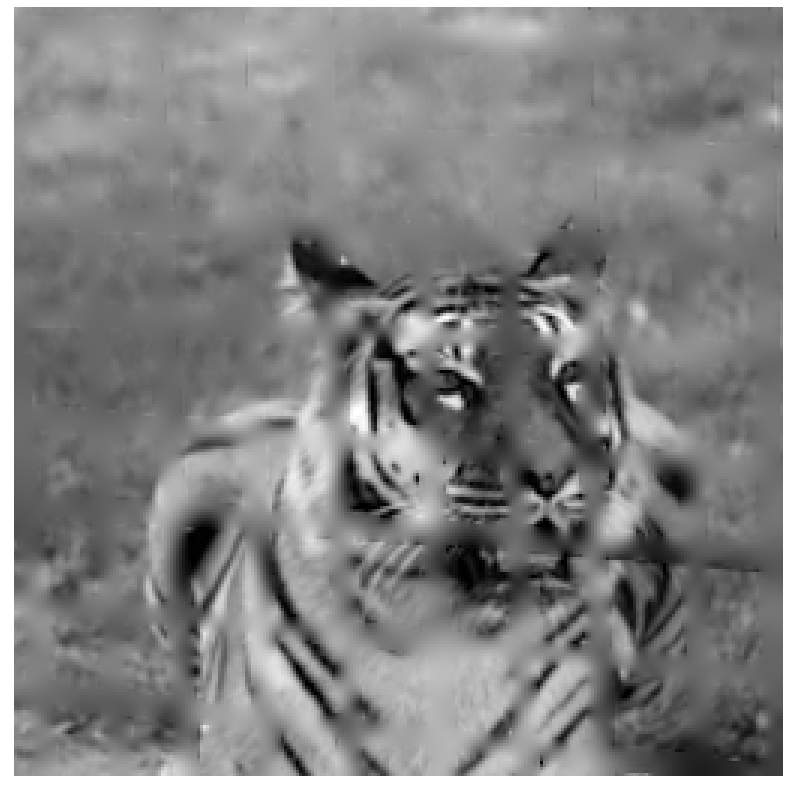
\includegraphics[width = .5\columnwidth]{fig/tigre_inpainting.png}
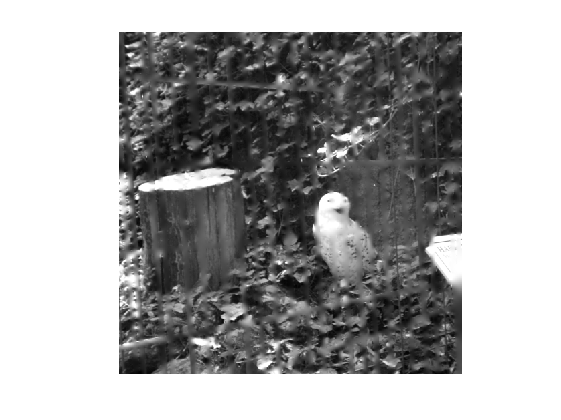
\includegraphics[width = .5\columnwidth]{fig/chouetteinpainting.png}
\end{tabular}
\caption{Inpainting sur des images naturelles après application du masque. La méthode est avec un seuillage doux et une base d'ondelettes orthogonales.}
\end{figure}






